\section{Making the robot move forward and backward}

\index{Parameter}We saw in chapter \ref{ch:proc-pascal} that a procedure
declaration gives a name to a sequence of commands that the
\robot\ can then execute once or several times when the procedure is called by its name.
A procedure can have one or several {\em parameters}. In that case the procedure
can perform actions that are similar but different when it is called with different
parameters.

For example the procedure
 {\idt fdn} (\underline{f}orwar\underline{d} \underline{n} times) tells the \robot\ to move straight ahead one
or several times by the length of the side of a square of the grid paper.
It has one parameter which gives the number of times the robot must move forward.
In \python, to call a procedure with a parameter, we write the name of the procedure followed
by the value of the parameter between parentheses.
`{\idt fdn(1)}' is equivalent to `{\idt fd()}' whereas
`{\idt fdn(4)}' is equivalent to `{\idt fd();\ fd();\ fd();\ fd()}'.
When the parameter is zero, the command `{\idt fdn(0)}' does not change the position of the \robot.
Finally, when the parameter is a negative number, that is to say a number preceded by the
minus sign $-$, the \robot\ moves backward the given number of times without changing its direction. For example
`{\idt fdn($-$4)}' is equivalent to `{\idt ht();\ fd();\ fd();\ fd();\ fd();\ ht()}'.

The parentheses must not be forgotten. If we write `{\idt fdn\ 4}', \python\ does not understand
and reports `{\tt SyntaxError: invalid syntax}'. If we write `{\idt fdn\ $-$4}', \python\
understands that we want to subtract 4 from {\idt fdn}, which makes no sense, and
reports during execution
`{\tt TypeError: unsupported operand type(s) for -: 'function' and 'int'}'
(an integer ({\idt int}) cannot be subtracted from a procedure ({\idt function})).
The parameter can also be an integer expression, as
in `{\idt fdn(2\ $\ast$\ j)}': \python\ first computes the value of the expression
{\idt 2\ $\ast$\ j} and then calls {\idt fdn} with this value.
If we forget the parameter, writing `{\idt fdn()}', \python\ reports
`{\tt TypeError: fdn() missing 1 required positional argument: 'n'}'
({\idt fdn()} is missing a required parameter) and if we give too many, as in
`{\idt fdn(1,\ 2)}', it reports
`{\tt TypeError: fdn() takes 1 positional argument but 2 were given}'
({\idt fdn()} takes one parameter but it was given two).

We can now understand the empty parentheses {\idt ()} that follow the commands
of the \robot\ we have used so far, such as {\idt fd()} or {\idt qtr()}:
in \python\ the parentheses order the call of the procedure, and they are empty
for procedures that need no information to run.
Beware: if we forget these empty parentheses, writing {\idt fd} instead
of {\idt fd()}, \python\ reports no error but the procedure is not called and the
\robot\ does not move forward!

\begin{exemple}{\rm
 The program {\idt OctagonalStripes} below draws the triangular stripes spread
 along the sides of an invisible octagon shown in figure \ref{fig:stries-oct}
 (page \pageref{fig:stries-oct}):\hfill
 \pagebreak[3]
 \input python/OctagonalStripes.tex
\noindent $\Box$ }\end{exemple}
\begin{figure}[htbp]
 \includevspacePostScript[6.0cm]{StriesOctogonales}{0.95}{0.95}
 \caption{Stripes on an octagon (scale $\frac{1}{3}$)}
 \label{fig:stries-oct}
\end{figure}

\section{Pen thickness}

The command {\idt pw} (\underline{p}en \underline{w}idth) sets the thickness of the pen of the \robot.
Its integer parameter gives the thickness of the pen
that is chosen. So far we have used a pen of thickness 1, which is the one the
\robot\ uses by default, that is to say when it is not told otherwise. The
command {\idt pw(2)} makes it draw with a line twice as thick. The unit of
length chosen to measure the thickness of the pen is the {\em pixel}, that is,
let us recall, the
size of the smallest dot that can be drawn on the computer screen.

When using a very thick pen, one must know that the pen of the \robot\
has a square tip and that the \robot\ holds this tip by its upper left corner.
\begin{center}
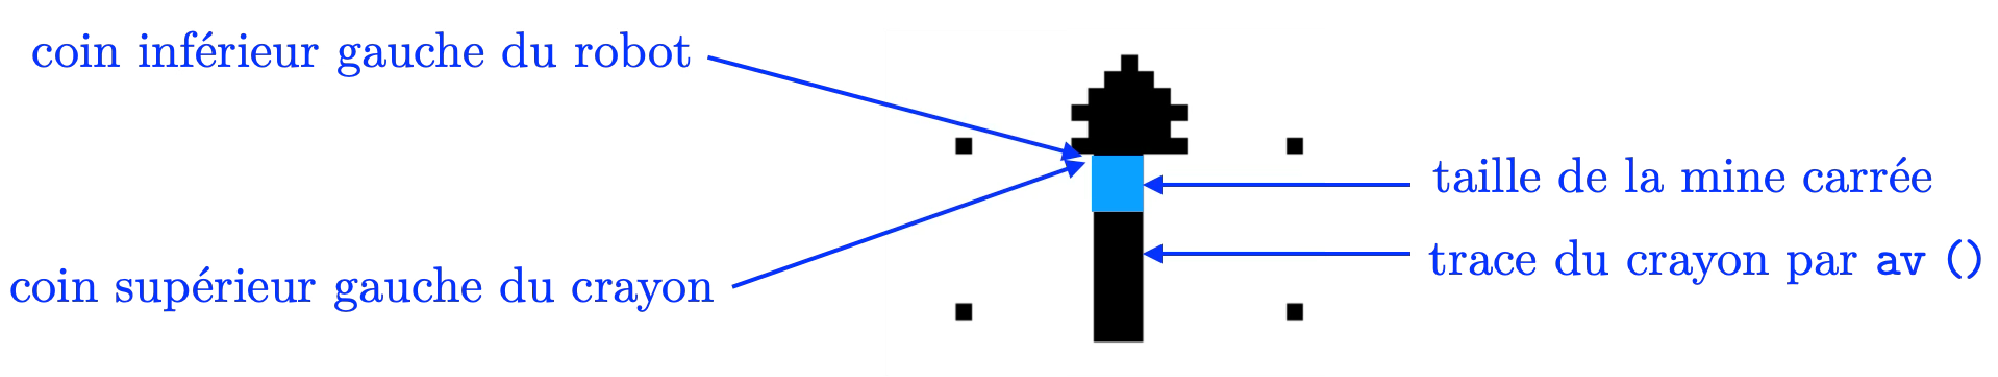
\includegraphics[width=0.9\textwidth]{ps-files/PositionTraceCrayon.pdf}
\end{center}

\begin{exemple}[Thick-tipped pen]{\rm
The program below, {\idt PenWidth}, lets us observe
 the effect of executing an {\idt fd()} command with a
 standard grid of 12 pixels when the \robot\ uses successive pen
 thicknesses of $12$, $24$, $36$ and $48$
 pixels:\par\nopagebreak
\noindent\begin{minipage}[t][6.4cm][t]{\linewidth}
\vspace*{6cm}%
\includePostScript{EpaisseurCrayon}{0.95}{0.95}%
\vspace*{-6cm}%
\input python/PenWidth.tex
\end{minipage}
We observe, for example, that the line drawn when the \robot\ executes
an {\idt fd()} command with a 48-pixel pen has an
apparent length of 5 times the length of the side of the grid. This
is explained by the fact that in its final position the pen leaves a
square mark with sides of $48$ pixels below and to the right of its stopping point,
that is $4$ times the length of the side of the $12$-pixel grid.
$\Box$ }%
\end{exemple}

\section{Speed of the robot}

A last example of a procedure with a parameter is the command {\idt sp} (\underline{sp}eed) to choose
the speed of the \robot. This speed is an integer between
0 and 10. Speed 10 corresponds to the default maximal speed. So the command {\idt sp(10)}
is equivalent to the command {\idt ex()} for normal execution. The speed
{\idt sp(1)} corresponds to the minimal speed. It lets us observe all the details of the
movements of the \robot\ which, at this speed, are very slow. Finally speed 0
corresponds to execution in step-by-step mode. The command {\idt sp(0)} is therefore equivalent
to the command {\idt ss()}. Step-by-step mode is used to find errors in
programs. In this mode of execution, the commands of the \robot\ are displayed at the bottom of the screen
and are executed by pressing a key (or by clicking the mouse button). The paths
of the \robot\ with the pen up are shown as dotted lines, which makes it possible to follow
its trail perfectly.

\needspace{6\baselineskip}\noindent \rule{137mm}{0.1mm}\par\nopagebreak %---------------------------------------------
\begin{exercices}{Write a \python\ program to draw:

\tiret the raised capital letter H of figure \ref{fig:h-relief} (page \pageref{fig:h-relief});

\tiret the cube in perspective, the eight-branched crystal and the pair of glasses of figure \ref{fig:crist+lun} (page \pageref{fig:crist+lun});

\tiret the helicopter and the passenger train of figure \ref{fig:transports} (page \pageref{fig:transports});

\tiret the `spirolateral' curves of figure \ref{fig:spiro} (page \pageref{fig:spiro}), obtained by making
the \robot\ move forward once, then twice, then three times, etc., turning each time a quarter turn to the right and repeating
the whole thing four times in a row (\cite{odds1});

\tiret the arabesque and the Jacob's ladder of figure \ref{fig:JacobArab} (page \pageref{fig:JacobArab}), a Jacob's ladder that you can also try to
make by weaving a string between your fingers.

\noindent $\Box$}\end{exercices}
\begin{figure}[htbp]
 \includevspacePostScript[2.6cm]{Cristal+Lunettes}{0.95}{0.95}
 \caption{Cube in perspective, eight-branched crystal and pair of glasses}
 \label{fig:crist+lun}
\end{figure}
\begin{figure}[htbp]
 \includevspacePostScript[4.0cm]{Spirolaterales}{0.95}{0.95}
 \caption{90$^{\circ}$ spirolaterals of order 5, 7 and 9}
 \label{fig:spiro}
\end{figure}
\begin{figure}[htbp]
 \includevspacePostScript[4.5cm]{JacobArab}{0.95}{0.95}
 \caption{Arabesque and Jacob's ladder}
 \label{fig:JacobArab}
\end{figure}


\begin{corrige} {\hfill
\input python/Spirolateral90degOrder9.tex
\noindent $\Box$}\end{corrige}
\nopagebreak
%%%%%%%%%%%%%%%%%%%%%%%%%%%%%%%%%%%%%%%%%%%%%%%%%%%%%%%%%%%%%%%%%%%%%%%%%%%
\noindent \framebox[\textwidth]{
\begin{minipage}{\myparboxwidth}
\setlength{\parindent}{2em}
\small \sf
\vspace{\abovedisplayskip}
\section*{Addenda}
The use of parameters in procedures is one of the basic notions of programming:
each call of the procedure depends on one or several values in terms of which
the effect of the procedure is expressed. For the time being we only consider parameter passing
{\em by value}, which allows information (one or several numbers in our case) to be passed
 to a procedure. This corresponds to the elementary notion of {\em function} (or {\em mapping})
in mathematics.

The use of subroutines with parameters in machine language is generally attributed to \href{https://en.wikipedia.org/wiki/Alan_Turing}{Alan Turing}.
The Swiss \href{https://en.wikipedia.org/wiki/Heinz_Rutishauser}{Heinz Rutishauser} \cite{rutishauser} and the Italian
\href{https://en.wikipedia.org/wiki/Corrado_Böhm}{Corrado Böhm} \cite{bohm} introduced the notions of high-level programming language and of compiler
to translate programs written in this high-level language into machine language (at the time people did not speak
of a compiler but of {\em automatic coding}). They included the notion of subroutine with parameters
in their languages without bringing it out very explicitly.

After these early theoretical contributions, the first compiler that actually worked, on the
{\sc mark i} machine in Manchester, England, was built by \href{https://en.wikipedia.org/wiki/Alick_Glennie}{Alick Glennie} in 1952. The high-level language
\href{https://en.wikipedia.org/wiki/Autocode}{{\sc autocode}} used subroutines with parameters passed in the registers of the machine.

\vspace{\abovedisplayskip}
\end{minipage}
}
%%%%%%%%%%%%%%%%%%%%%%%%%%%%%%%%%%%%%%%%%%%%%%%%%%%%%%%%%%%%%%%%%%%%%%%%%%%%

%%%%%%%%%%%%%%%%%%%%%%%%%%%%%%%%%%%%%%%%%%%%%%%%%%%%%%%%%%%%%%%%%%%%%%%%%%%
\noindent \framebox[\textwidth]{
\begin{minipage}{\myparboxwidth}
\setlength{\parindent}{2em}
\small \sf
\vspace{\abovedisplayskip}
This work
had no success because programming was relatively easy at the time compared with the effort
needed to adapt programs to the malfunctions of the machine.
\href{https://en.wikipedia.org/wiki/Maurice_Wilkes}{Maurice Wilkes} \cite{wilkes1} introduced
 the use of li\-brar\-ies of procedures (like the ones we use for the commands of the \robot) in 1951.

 The first language in which these notions appeared in their modern form was \href{https://en.wikipedia.org/wiki/Fortran}{\sc fortran} ({\sc for}mula
 {\sc tran}slator), designed in 1954 by a team led by \href{https://en.wikipedia.org/wiki/John_Backus}{John Backus} \cite{fortran}. Thanks to very
 many modifications incorporating new programming concepts,
 to extensions taking into account
 recent machine architectures and to the wealth of available libraries,
 this language is still widely used for numerical scientific programming.

\vspace{\abovedisplayskip}
\end{minipage}
}
%%%%%%%%%%%%%%%%%%%%%%%%%%%%%%%%%%%%%%%%%%%%%%%%%%%%%%%%%%%%%%%%%%%%%%%%%%%%
\newpage
\thispagestyle{empty}
